\subsection{Identity-Transformation Algorithms}
\label{subsec:overview}

We design identity-transformation algorithms %  $\mathcal{F}_{PID_{RP}}$, $\mathcal{F}_{PID_{U}}$ and $\mathcal{F}_{Acct}$,
on an elliptic curve $\mathbb{E}$.
Table \ref{tbl:notations-protocol} lists the notations. The subscript $j$ and/or superscript $i$ may be omitted if there is no ambiguity.


\begin{table}[tb]
\footnotesize
    \caption{Notations used in the \usso protocol}
    \centering
%    \begin{tabular}{|c|c|c|}
    \begin{tabular}{|p{0.93cm}|p{6.71cm}|} \hline
    {\textbf{Notation}} & {\textbf{Description}} \\ \hline
    {$\mathbb{E}$, $G$, $n$} & {$\mathbb{E}$ is an elliptic curve over a finite field $\mathbb{F}_q$. $G$ is a base point (or generator) on $\mathbb{E}$, and the order of $G$ is a prime number $n$.} \\ \hline
    {$ID_U$} & {$ID_U = u \in [1, n)$ is the user's unique identity at the IdP, \newc{which is known only to the user and the IdP. %$u$ is kept unknown to RPs.
    }} \\ \hline
   {$ID_{RP_j}$} & {$ID_{RP} = [r]G$ is the $j$-th RP's unique identity, which is publicly known; $r \in [1, n)$ \newc{is known only to the IdP but not the RP.}} \\ \hline
    {$t$} & {$t \in [1, n)$ is a user-selected random integer in each login; \newc{$t$ is shared with the target RP and kept secret to the IdP.
    }} \\ \hline
    {$PID_{RP_j}^i$} & {$PID_{RP} = [t]{ID_{RP}} = [tr]G$ is the $j$-th RP's pseudo-identity, in the user's $i$-th login to this RP.} \\ \hline
    {$PID_{U,j}^i$} & {$PID_U = [{ID_U}]{PID_{RP}} = [utr]G$ is the user's pseudo-identity, in the user's $i$-th login to the $j$-th RP.} \\ \hline
     {$Acct_j$} & {$Acct = [t^{-1}\bmod n]PID_{U} = [ID_U]ID_{RP} = [ur]G$ is the user's account at the $j$-th RP.} \\ \hline
    {$SK$, $PK$} & {The IdP's private key and public key, which are used to sign and verify identity tokens and RP certificates.} \\ \hline
%    {$T$} & {The trapdoor to derive $Account$: $T=N_U^{-1} \bmod n$.} \\ \hline
    {$Enpt_{RP_j}$} & {The $j$-th RP's endpoint for receiving the identity tokens.} \\ \hline
    {$Cert_{RP_j}$} & {The IdP-signed RP certificate binding $ID_{RP_j}$ and $Enpt_{RP_j}$.} \\ \hline
%    {$PEnpt_{U,j}^i$} & {A user-generated random "pseudo-endpoint'', in the user's $i$-th login to the $j$-th RP.} \\ \hline
    \end{tabular}
    \label{tbl:notations-protocol}
\end{table}

The IdP assigns a unique random integer $u$ to a user (i.e., $ID_U = u$),
 while selecting a random integer $r$ and assigning $ID_{RP} = [r]G$ to the RP if it is a unique point on $\mathbb{E}$.
Here, $G$ is a point on $\mathbb{E}$ of order $n$, and $[r]G$ denotes the addition of $G$ on the curve $r$ times.


%The IdP assigns a unique random integer $u$ to a user (i.e., $ID_U = u$). When an RP registers, the IdP generates a random number $r$ and assigns $ID_{RP} = [r]G$, which is a unique point on $\mathbb{E}$.
%Here, %$u, r \in [1,n)$, %$r$ is unknown to the RP, and
%$[r]G$ is the addition of $G$ on the curve $r$ times.

%\vspace{0.5mm}

\noindent {\bf $\boldsymbol{ID_{\boldsymbol{RP}}}$-$\boldsymbol{PID_{\boldsymbol{RP}}}$ Transformation.} A user selects a random number $t \in [1, n)$ as the trapdoor and calculates $PID_{RP}$.
\begin{equation}
PID_{RP} = \mathcal{F}_{PID_{RP}}(ID_{RP}) = [t]{ID_{RP}} = [tr]G
\label{equ:PIDRP}
\end{equation}
\newc
In each login, the user selects $t$ and shares it with the RP to negotiate $PID_{RP}$.
It makes no difference if the RP selects $t$ randomly and sends it to the user, as long as both of them calculate $PID_{RP}$ independently and check if the received $PID_{RP}$ is equal to the calculated one.

\oldc
\noindent {\bf $\boldsymbol{ID_U}$-$\boldsymbol{PID_U}$ Transformation.}
On receiving an identity-token request with $ID_U$ and $PID_{RP}$, the IdP calculates $PID_{U}$.
\begin{equation}
PID_{U} = \mathcal{F}_{PID_U}(ID_U, PID_{RP}) =
  [{ID_U}]{PID_{RP}} = [utr]G
 \label{equ:PIDU}
\end{equation}


\noindent {\bf $\boldsymbol{PID_U}$-$\boldsymbol{Acct}$ Transformation.}
The trapdoor $t$ is sent to the target RP, which checks whether $PID_{RP}$ included in identity tokens equals $[t]ID_{RP}$. After verifying a token that binds $PID_U$ and $PID_{RP}$, it calculates $Acct$ as follows.
\begin{equation}
Acct = \mathcal{F}_{Acct}(PID_{U})
   = [t^{-1} \bmod n]PID_{U}
   \label{equ:Account}
\end{equation}
From Equations \ref{equ:PIDRP}, \ref{equ:PIDU}, and \ref{equ:Account}, it is derived that
\begin{equation}
   Acct =  [t^{-1}utr \bmod n]G = [ur]G = [ID_U]ID_{RP}
   \label{equ:AccountNotChanged}
\end{equation}
%<<<<<<< HEAD
%With the help of $t$, the RP can derive an \emph{identical permanent} account from the identity tokens in different logins. %from the user.
%The accounts at different RPs are unique for a given user, while the accounts of different users are unique for a given RP. The RP cannot derive $ID_U$ from either $PID_U$ or $Acct$ due to the elliptic curve discrete logarithm problem (ECDLP). Since $t$ is random in $\mathbb{Z}_n$ and unknown to the IdP, from the IdP's view, $PID_{RP}$ is indistinguishable from a random variable on $\mathbb{E}$. So, the IdP cannot learn anything about $ID_{RP}$ from $PID_{RP}$.
%%Section \ref{sec:analysis} presents more detailed analyses.
%Note that $r$ should be kept secret to the RP; otherwise, two colluding RPs with $ID_{RP_j} = [r]G$ and $ID_{RP_{j'}} = [r']G$ could link a user's accounts by checking if $[r']Acct_j = [r]Acct_{j'}$ holds.
%
%\textcolor{blue}{A user and an RP negotiate $PID_{RP} = [t]ID_{RP}$ by selecting a random number $t$ and keeping it secret between them. They need to calculate $PID_{RP}$ independently. In particular, when one party selects $t$ and computes $PID_{RP} = [t]ID_{RP}$, the other party should check if the received $t$ and $PID_{RP}$ satisfies $PID_{RP} = [t]ID_{RP}$. In our protocol, we ask the user to generate $t$, compute $PID_{RP}$, and send them to the RP. %In the above descriptions, the user generates $t$, calculates $PID_{RP} = [t]ID_{RP}$ and sends $t$ to the RP. After receiving $t$ from the user and extracting $PID_{RP}$ from a token, the RP checks that $PID_{RP} = [t]ID_{RP}$, because the correct account $[ID_U]ID_{RP}$ is derived \emph{only if} this equation holds (i.e., $PID_{RP} = [t]ID_{RP}$); otherwise, attacks happen as below.
%The RP should compute $[t]ID_{RP}$ by itself and verify if it equals the received $PID_{RP}$. Otherwise, a malicious user with $ID_{U'} = u'$ could impersonate a victim user with $ID_{U} = u$ who holds $Acct$ at that RP, if he uses $[t'u'^{-1}]Acct$ as $PID_{RP}$ to request an identity token from the IdP. The IdP would calculate $PID_{U'} = [u'][t'u'^{-1}]Acct = [t']Acct$, with which the RP would authenticate the malicious user under $Acct$.
%% To login as any $Acct$,
%%         a malicious user with $ID_{U'} = u'$ could generate a random number $t'$,
%%             and calculate $[t'u'^{-1}]Acct$ as $PID_{RP}$ to request an identity token.
%% Then, the IdP will calculate $PID_{U'} = [u'][t'u'^{-1}]Acct = [t']Acct$.
%% Without checking $PID_{RP} = [t']ID_{RP}$ or not,
%%         the RP will finally allow the malicious user to login as $[t'^{-1}]PID_{U'} = Acct$.
%}
%
%\textcolor{blue}{Meanwhile, if the RP selects $t$ and calculates $PID_{RP}$, the user should compute $[t]ID_{RP}$ by herself and check if $PID_{RP} = [t]ID_{RP}$ holds. Otherwise, a malicious user $ID_{U'}$ could collude with a malicious $RP'$ to impersonate the victim user at the honest $RP$. Assume $ID_{U'}$ receives $PID_{RP}=[t']ID_{RP}$ from the honest $RP$ and forwards it to the victim user through the malicious $RP'$ in another login. If the victim user does not check if the received $PID_{RP}$ equals to $[t']ID_{RP'}$, she would request an identity token that binds $PID_U$ and $PID_{RP}$ from the IdP and presents it to the malicious RP. This token would allow the malicious user to log in to the honest RP on behalf of the victim user.
%% Then $U'$ colludes with a malicious RP denoted as $RP'$,
%%     which intentionally sends $PID_{RP}$ to an honest user $U$ in some login.
%% Without checking $PID_{RP} = [t']ID_{RP'}$ or not,
%%     this honest user will present a token binding $PID_U$ and $PID_{RP}$ to $RP'$.
%% Finally, this token enables malicious $U'$ to log in as the honest user's account at the honest RP.
%}
%%In other words, this checking ensures RP designation,
%%    because it is impossible to find $t$ and $t'$ satisfying that
%%    $[t]ID_{RP} = [t']ID_{RP'}$,
%%        when $ID_{RP} = [r]G$, $ID_{RP'} = [r']G$, but $r$ and $r'$ are unknown.
%%See Section \ref{sec:analysis} for the detailed proofs of security and privacy.
%

With the help of $t$, for a given user, the RP derives an \emph{identical} account from identity tokens for different logins. It is the user's \emph{permanent} account at this RP, which is \emph{unique} among all accounts at the same RP. Meanwhile, the user's accounts at different RPs are inherently different and unlinkable (see Section \ref{sec:analysis} for the detailed proof).

\newc
In this process, the RP needs to check if $PID_{RP} = [t]ID_{RP}$ holds after extracting $PID_{RP}$ from a received identity token. Otherwise, a malicious user with $ID_{U'} = u'$ could randomly select $t'$ and $u$, and set $PID_{RP}$ as $[t'u'^{-1}][u]ID_{RP}$. Then, the malicious user requests a token from the IdP, in which $PID_{U'} = [ID_{U'}]PID_{RP}=[u'][t'u'^{-1}][u]ID_{RP} = [t'u]ID_{RP}$.
If the RP does not check the received $PID_{RP}$, it would use the received $PID_{U'}$ to calculate an account as $Acct = [t'^{-1}]PID_{U'}=[u]ID_{RP}$, which is the account of a potential victim user with $ID_{U} = u$.
The malicious user could repeat the above attacks with random $u \in \mathbb{Z}_n$ until the account of some victim user is calculated by the RP.\footnote{\newc If it does not derive an existing account of some honest user, the RP will treat the adversary as a newly-registered user without any alerts.}

%Otherwise, a malicious user with $ID_{U'} = u'$ could impersonate a victim user by setting $PID_{RP}$ to $[t'u'^{-1}]Acct$ but sending $t'$ to an RP, where $Acct$ belongs to the victim with $ID_{U} = u$ at this RP.
%Then, the malicious user could request an identity token, and the IdP would calculate $PID_{U'} = [u'][t'u'^{-1}]Acct = [t']Acct$.
%Finally, the RP would accept the malicious user under $Acct$. %In particular, when one party selects $t$ and computes $PID_{RP} = [t]ID_{RP}$, the other party should check if the received $t$ and $PID_{RP}$ satisfies $PID_{RP} = [t]ID_{RP}$.
%In the above descriptions, the user generates $t$, calculates $PID_{RP} = [t]ID_{RP}$ and sends $t$ to the RP. After receiving $t$ from the user and extracting $PID_{RP}$ from a token, the RP checks that $PID_{RP} = [t]ID_{RP}$, because the correct account $[ID_U]ID_{RP}$ is derived \emph{only if} this equation holds (i.e., $PID_{RP} = [t]ID_{RP}$); otherwise, attacks happen as below.
%The RP should compute $[t]ID_{RP}$ by itself and verify if it equals the received $PID_{RP}$.

Similarly, if the RP selects $t$ and calculates $PID_{RP}$, the user needs to check whether the received $PID_{RP}$ equals $[t]ID_{RP}$ before requesting an identity token.
Otherwise, malicious users could impersonate a victim user at some honest RP by colluding with another malicious RP.
That is, when receiving $PID_{RP}=[t']ID_{RP}$ from the honest RP, the malicious user forwards it to $RP'$, which sends it to the victim user in another login.
If the victim does not check the received $PID_{RP}$, she would request from the IdP an identity token that binds $PID_U$ and the manipulated $PID_{RP}$ and present the token to the malicious RP.
This token would allow the malicious user to log into the honest RP under the victim user's account.

\oldc
The IdP never discloses $r$ to RPs; otherwise, two colluding RPs with $ID_{RP_j} = [r]G$ and $ID_{RP_{j'}} = [r']G$ could link a user's accounts by checking whether $[r']Acct_j = [r]Acct_{j'}$ holds.
\newc
In the meantime, a user's identity $u$ is kept secret to RPs; otherwise, colluding RPs could enumerate the user's accounts by calculating $[u]ID_{RP_j}$ and then link them.
\oldc

%======move to security analysis
%The RP cannot derive $ID_U$ from either $PID_U$ or $Acct$ due to the elliptic curve discrete logarithm problem (ECDLP). Since $t$ is random in $\mathbb{Z}_n$ and unknown to the IdP, from the IdP's view, $PID_{RP}$ is indistinguishable from a random variable on $\mathbb{E}$. So, the IdP cannot learn anything about $ID_{RP}$ from $PID_{RP}$.
%Section \ref{sec:analysis} presents more detailed analyses.


\subsection{The Design Specifics for Web Applications}
\label{sec:web-design}

In commonly-used SSO protocols \cite{OpenIDConnect,rfc6749, SAML, SAMLIdentifier},
an IdP needs to know the visited RP to ensure the \emph{confidentiality} of identity tokens. For instance, in OIDC services, an RP's endpoint to receive tokens is stored as the \verb+redirect_uri+ parameter at the IdP.
The IdP employs HTTP 302 redirection to send identity tokens to the RP, by setting this parameter as the target URL in the HTTP responses to a user's identity-token request \cite{OpenIDConnect}, so the user agent forwards it to the designated RP.
However, in \usso, the IdP does not know about the visited RPs, requiring a user agent by itself to calculate $PID_{RP}$ and send identity tokens to the RP's endpoint.
%In UPPRESSO, the IdP is not aware of visited RPs, so user agents (or browsers) are responsible for forwarding the identity token to the intended RP and computing $PID_{RP}$. On the contrary, in commonly-used SSO protocols \cite{OpenIDConnect,rfc6749,SAML,SAMLIdentifier}, the IdP requires this information to ensure the \emph{confidentiality} of identity tokens. For instance, in OIDC services, an RP's endpoint URL is set as the \verb+redirect_uri+ parameter \cite{OpenIDConnect} during registration to receive tokens. When transmitting identity tokens to an RP, the IdP employs HTTP 302 redirection. This endpoint is the target URL in HTTP responses, allowing the browser to forward it to the designated RP.

\usso\ supports commercial-off-the-shelf (COTS) browsers to work as the user agent and implements the user-agent functions using web scripts in browsers. The scripts are responsible for communications with the origin web servers,
 and downloaded from the IdP and the visited RP, respectively. It is worth noting that a script downloaded from an honest entity is considered \emph{honest}.

The IdP script is necessary because the RP script could leak its origin to the IdP web server due to the automatic inclusion of an HTTP \verb+referer+ header in all HTTP requests it sends.
Besides, the IdP script is trusted to interact with the users for attribute authorization,
 %and ensure the confidentiality of identity tokens, i.e., a token is sent to only the designated RP,
%% 机密性这一句没有必要写,因为“如果RP是malicious,则RP总是可以将token泄露出去”。
  while the RP (and its script) could be malicious.
Thus, on receiving an identity-token request, the IdP web server checks the \verb+referer+ header to ensure it is sent by the IdP script.

%Section \ref{sec:discussion} discusses more efficient but less portable implementations with browser extensions.

The RP script is responsible for preparing $ID_{RP}$ and $Enpt_{RP}$ for the IdP script through an RP certificate issued by the IdP. %It binds the RP's identity and endpoint. %(i.e., $ID_{RP}$ and $Enpt_{RP}$).
In each login, the RP script sends the certificate to the IdP script, which then verifies it and extracts $ID_{RP}$ and $Enpt_{RP}$.
The same as in widely-adopted SSO systems \cite{OpenIDConnect, rfc6749, SAML, SAMLIdentifier}, in \usso\ a user does not need to configure anything locally as the IdP's public key is already set in the IdP script.

After receiving an identity token from the IdP, the IdP script needs to ensure the RP script will forward the token to $Enpt_{RP}$ %, which is bound with $ID_{RP}$
specified in the RP certificate.
As the communication between the scripts occurs within the browser using the \verb+postMessage+ HTML5 API, %To avoid the honest user sending the identity token to an adversary,
we use the \verb+postMessage+ targetOrigin mechanism \cite{postm-targeto} to restrict the recipient. %(i.e., the RP script).
 When the IdP script sends messages, the recipient's origin is set as a parameter, such as \verb+postMessage(tk, 'https://RP.com')+, which includes the protocol (e.g., \verb+https+), the domain (e.g., \verb+RP.com+), and a port if applicable.
Only the script downloaded from this targetOrigin is considered a legitimate recipient.

%The \emph{RP certificates} deals with the problem of mapping an identity proof with its targeting RP.
%That is, the IdP script derives the RP's $ID_{RP}$ and origin from the RP certificate, while the $PID_{RP}$ is generated with this $ID_{RP}$. Thus, the IdP script always knows the targeting RP of identity proof, therefore, the \verb+postMessage+ mechanism can guarantee that the identity proof would not be sent to the adversary.

\newc
As discussed in Section \ref{subsec:overview}, a user needs to by herself calculate $PID_{RP} = [t]ID_{RP}$ based on $ID_{RP}$ extracted from the RP certificate. Thus, this function should be implemented by an \emph{honest} script that does not leak $t$ to the IdP, from which it could calculate $ID_{RP} = [t^{-1}\bmod n]PID_{RP}$. In \usso, we consider the IdP script honest; otherwise, it could directly leak the RP's domain to the IdP.
To mitigate this risk, we can implement the user agent with trusted browser extensions, which need to be installed by users before visiting RPs.
\oldc

\begin{figure*}[htb]
  \centering
  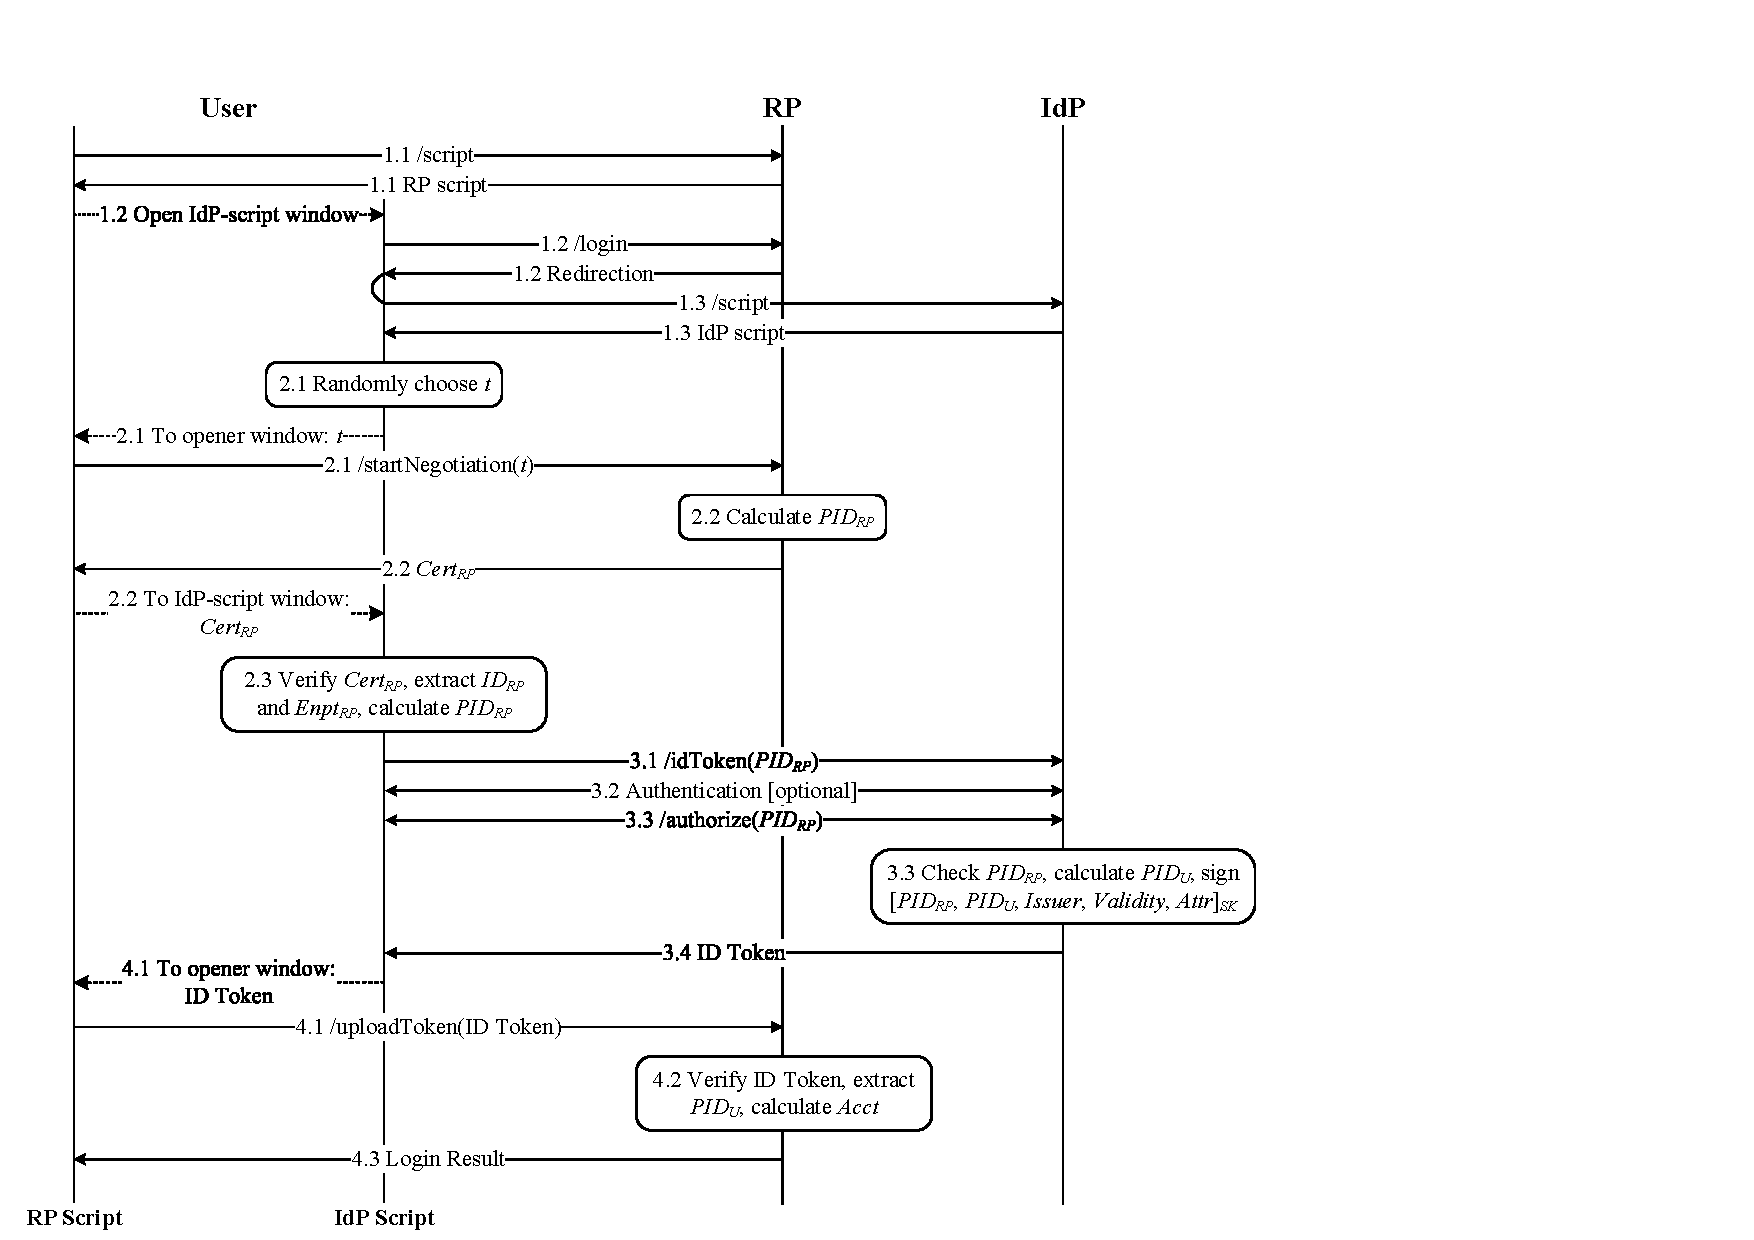
\includegraphics[height=0.5591\textheight]{fig/process-js.pdf}
  \caption{The SSO login flow of \usso}
  \label{fig:process}
\end{figure*}

When a user is visiting an RP, the browser downloads the RP script, which in turn opens a new window to download the IdP script. To prevent referer leakage during the download of the IdP script, we need to ensure that the HTTP request does not automatically carry a \verb+referer+ header, which reveals the visited RP's domain to the IdP. %Generally, when a browser window visits another website not belonging to its opener's origin, the HTTP request to this website automatically carries a \verb+referer+ header (i.e., the opener's origin). Such an HTTP header leaks the visited RP's domain to the IdP.
In \usso, this new window is a \emph{redirection} from the RP to the IdP (Figure \ref{fig:process}, Steps 1.2-1.3), not a direct visit by the browser.
The HTTP response from the RP includes a \verb+referrer-policy=no-referrer+ header, which ensures that the HTTP request to download the IdP script carries no \verb+referer+ header.
This approach is specified by W3C \cite{referer_policy} and widely supported. We have tested it in various browsers such as Chrome, Safari, Edge, Opera, and Firefox, and confirmed that no referer leakage occurs.




\subsection{The \usso\ protocol}
\label{implementations}

\noindent \textbf{System Initialization.}
An IdP generates a key pair ($SK$, $PK$) to sign and verify identity tokens and RP certificates.
%The IdP keeps $SK$ secret, and $PK$ is publicly known.

\vspace{1.5mm}
\noindent\textbf{RP Registration.}
%Each RP launches an initial registration operation to finish configurations.
Each RP registers itself at the IdP to obtain $ID_{RP}$ and its RP certificate $Cert_{RP}$ as follows:
\vspace{-\topsep}\begin{enumerate}
\setlength{\topsep}{0pt}
\setlength{\partopsep}{0pt}
\setlength{\itemsep}{0pt}
\setlength{\parsep}{0pt}
\setlength{\parskip}{0pt}
\item
An RP pre-installs $PK$ by trusted means.
It sends a registration request, including the endpoint to receive identity tokens and other information.
\item
The IdP selects a random number $r \in [1,n)$ until $ID_{RP} = [r]G$ is unique.
 %   but $r$ is kept unknown to the RP.
It signs $Cert_{RP} = [ID_{RP}, Enpt_{RP}, *]_{SK}$,
     where $[\cdot]_{SK}$ is a message signed using $SK$ and $*$ is supplementary information such as the RP's common name.
\item
The RP verifies $Cert_{RP}$ using $PK$ and accepts $ID_{RP}$ and $Cert_{RP}$ if they are valid.
\end{enumerate}


%\vspace{0.5mm}
\noindent\textbf{User Registration.}
Each user registers once at the IdP. She sets up a unique random identity $ID_U = u \in [1, n)$ and the corresponding credential. $ID_U$ is kept unknown to RPs.
%This is similar to the steps in existing SSO systems.


\vspace{1.5mm}
\noindent\textbf{SSO Login.} A login %is typically launched through a browser,
%when a user attempts to visit an RP. It
involves four steps: script downloading, RP identity transformation, identity-token generation, and $Acct$ calculation. In Figure \ref{fig:process}, the IdP's and RP's operations are connected by two vertical lines, respectively. The user operations are split into two groups in different browser windows by two vertical lines, one communicating with the IdP and the other with the RP. Solid horizontal lines indicate messages exchanged between the user and the IdP (or the RP), while dotted lines represent a \verb+postMessage+ invocation between two scripts (or browser windows) within the browser.


\vspace{0.85mm}
\noindent 1. {\em Script Downloading.}
The browser downloads scripts from the visited RP and the IdP.
\vspace{-\topsep}
\begin{itemize}
\setlength{\topsep}{0pt}
\setlength{\partopsep}{0pt}
\setlength{\itemsep}{0pt}
\setlength{\parsep}{0pt}
\setlength{\parskip}{0pt}
\item[1.1]
When requesting any protected resources at the RP, the user downloads the RP script.
\item[1.2]
The RP script opens a window in the browser to visit the login path at the RP, which is then redirected to the IdP.
\item[1.3]
The redirection to the IdP downloads the IdP script.
\end{itemize}



%\vspace{1mm}
\noindent 2. {\em RP Identity Transformation.}
The user and the RP negotiate $PID_{RP} = [t]{ID_{RP}}$.
\vspace{-\topsep}
\begin{itemize}
\setlength{\topsep}{0pt}
\setlength{\partopsep}{0pt}
\setlength{\itemsep}{0pt}
\setlength{\parsep}{0pt}
\setlength{\parskip}{0pt}
\item[2.1] The IdP script chooses a random number $t \in [1, n)$ and sends it to the RP script through \verb+postMessage+. The RP script then forwards $t$ to the RP.
\item[2.2] The RP verifies if the received $t$ is an integer in $[1, n)$ and
%Upon receiving $t$, the RP verifies $1 \leq t < n$ and %calculates $PID_{RP}$.
%To acknowledge the negotiation of $PID_{RP}$, The RP
replies with $Cert_{RP}$ and the scope of the requested user attributes. The reply is transmitted through the RP script to the IdP script.  % through \verb+postMessage+.
\item[2.3] The IdP script verifies $Cert_{RP}$, extracts $ID_{RP}$ and $Enpt_{RP}$ from $Cert_{RP}$, and calculates $PID_{RP}=[t]{ID_{RP}}$.
%It then creates a random endpoint $PEnpt_{U}$ for this login,
 %   to receive identity tokens from the IdP.
    % as the RP endpoint required by IdP.我们已经修改了协议, IdP并不require什么

\end{itemize}


%\vspace{1mm}
\noindent 3. {\em Identity-Token Generation.}
The IdP calculates $PID_U = [ID_U]{PID_{RP}}$ and signs an identity token. % The processes are as follows.
\vspace{-\topsep}
\begin{itemize}
\setlength{\topsep}{0pt}
\setlength{\partopsep}{0pt}
\setlength{\itemsep}{0pt}
\setlength{\parsep}{0pt}
\setlength{\parskip}{0pt}
\item[3.1]
The IdP script sends an identity-token request for $PID_{RP}$ on behalf of the user. %and the user attributes.
 %by checking whether this user is authenticated by IdP.

\item[3.2] The IdP authenticates the user, if not authenticated yet.

\item [3.3]
The IdP script obtains the user's authorization for the requested attributes locally and then sends the scope of the authorized attributes.
\newc
Then, the IdP checks if the received $PID_{RP}$ is a point on $\mathbb{E}$,
\oldc
calculates $PID_U = [ID_U]{PID_{RP}}$, and signs $[PID_{RP}, PID_U, Issuer, Validity, Attr]_{SK}$, where $Issuer$ is the IdP, $Validity$ indicates the validity period, and $Attr$ contains the authorized user attributes.
\item[3.4] The IdP replies with the identity token to the IdP script.
\end{itemize}

%\vspace{1mm}
\noindent 4. {\em $Acct$ Calculation.}
The RP receives the identity token and authorizes the user to log in.
\vspace{-\topsep}
\begin{itemize}
\setlength{\topsep}{0pt}
\setlength{\partopsep}{0pt}
\setlength{\itemsep}{0pt}
\setlength{\parsep}{0pt}
\setlength{\parskip}{0pt}
\item [4.1]
The IdP script forwards the identity token to the RP script,
    which sends it to the RP through $Enpt_{RP}$.
\item[4.2] The RP verifies the identity token by checking the IdP's signature and its validity period.
Then, \newc
the RP extracts $PID_{RP}$ from the token, checks if it equals $[t]ID_{RP}$,
\oldc
and calculates $Acct = [t^{-1}]{PID_U}$.

\item [4.3] The RP authorizes the user to log in as $Acct$.

\end{itemize}


If any verification fails, this flow will be terminated immediately.
For example, the user halts it when receiving an invalid $Cert_{RP}$.
\newc
The IdP rejects an identity-token request in Step 3.3 if the received $PID_{RP}$ is not a point on $\mathbb{E}$, and the RP rejects an identity token in Step 4.2 if the signature is invalid or the enclosed $PID_{RP}$ is not equal to $[t]ID_{RP}$.
\oldc


\subsection{Compatibility with OIDC}
\label{subsec:compatible}

Both \usso\ and OIDC work with COTS browsers. %Among the four steps of the login flow
In \usso, the \emph{script downloading} step prepares the user agent, which assists the communications with the IdP and RP servers. \usso\ employs web scripts to hide the RP's endpoint from the IdP, while securely forwarding identity tokens to the RP through $Enpt_{RP}$ extracted from the signed RP certificate.
% that protects the identity token from being sent to adversaries. 这句话与Compatibility无关
Therefore, the IdP does not set \verb+redirect_uri+ in the HTTP responses, which is different from OIDC where HTTP redirections are used to implement these communications. Most operations in the \emph{RP identity transformation} step take place within browsers. The RP only receives $t$ to generate an RP pseudo-identity and responds with $Cert_{RP}$,
%The calculation of $PID_{RP}$ is viewed as the operation to prepare an RP identity in OIDC,
which is viewed as a supplementary message to users.
%The operations in the $PID_{RP}$ registration are almost identical to those in the RP Dynamic Registration of OIDC \cite{DynamicRegistration}, except that in OIDC the IdP assigns the RP's identity  while in UPPRESSO this (pseudo-)identity is generated by the registered entity. Besides, the $PID_{RP}$ registration has a validity period.
Consequently, compared to the original OIDC protocol, \usso\ simplifies the IdP's operations in these two steps, while allowing RPs to customize their ``dynamic'' pseudo-identities.

The operations of \emph{identity-token generation} and \emph{$Acct$ calculation} in \usso\ are \emph{identical} to those in OIDC,
 because (\emph{a}) the calculation of $PID_U$ in \usso\ can be viewed as a method to generate PPIDs in OIDC and (\emph{b}) the calculation of $Acct$ can be viewed as a mapping from the user identity in tokens to an account at the RP.

The compatibility is experimentally confirmed through our prototype implementation, which modifies only 23 lines of Java code in MITREid Connect \cite{MITREid}, an open-source OIDC system, to build an IdP in \usso\ (see Section \ref{subsec:proto-imple}).
%It will help the adoption and deployment of UPPRESSO.

